\chapter{Proposta}
\label{cap:proposta}

Nesta seção é detalhada a proposta de modelo adaptativo a ser desenvolvido de percepção veicular de ambiente e propriocepção veicular. Nas próximas seções é detalhada a metodologia e materiais adotados, andamento da pesquisa, resultados preliminares obtidos e cronograma de atividades.

\section{Metodologia}

Para o desenvolvimento deste trabalho, inicialmente foi realizado o levantamento do estado-da-arte sobre percepção veicular de ambiente e propriocepção veicular, através de sinais de sensores inerciais. Este levantamento se deu por intermédio de produção de uma Revisão Sistemática da Literatura (RSL), em bases de dados relevantes na área de computação. Através dessa sistemática, diversas lacunas de pesquisa foram identificadas conforme discorrido no capítulo \ref{cap:revisao}, com a delimitação de escopo desta pesquisa. Baseando-se nas lacunas de pesquisa, o desenvolvimento da metodologia de percepção adaptativa se dá em três etapas, sendo elas a coleta de dados, o pré-processamento e processamento. 

Na etapa de de coleta de dados, são utilizadas duas redes de sensores no veículo, sendo cada uma destas constituídas por um \textit{Single-Board Computer} (SBC) Raspberry Pi e três placas MPU-9250, cada uma equipada com um acelerômetro, um giroscópio e um magnetômetro. Também foi utilizado uma fonte externa de GPS, com produção de dados de localização e velocidade. Para definição dos referenciais, utilizou-se posicionamento controlado, uma vez que melhor se adéqua ao estudo. Sendo assim, o posicionamento das placas foi realizado de forma que os eixos do referencial do sensor coincidem com os do veículo, não sendo necessário mapear. As redes com as placas MPU-9250 foram distribuídas no veículo de forma a considerar os dados provindos de pontos com diferentes fatores de dependência, uma vez que a análise busca estabelecer qual ponto fornece os dados que produzem melhores resultados. Sendo assim, foram distribuídas no veículo da seguinte maneira: cada extremidade do eixo frontal (lado direito e esquerdo) recebeu uma das redes, onde anexou-se uma placa na bandeja da suspensão, localizando-se abaixo e próximo à suspensão veicular; outra placa acima e próxima à suspensão, anexada na lataria; e outra placa anexada na \textit{dashboard} do veículo, dentro da cabine. A taxa de amostragem não foi restringida, atingindo próximo a 1 kHz, uma vez que para os experimentos será realizado \textit{downsampling} para verificar a melhor taxa. Foi empregada a faixa de medição máxima (8g), uma vez que em testes exploratórios foi observado em algumas ocasiões a produção de valores de até aproximadamente 7.5g. 

Após, na etapa de pré-processamento se busca melhorar os dados brutos antes de serem parametrizados a técnica de reconhecimento de padrões. Sendo assim, será utilizada técnica empregada por \cite{Li2018} para aproximar as localizações e velocidade em uma taxa próxima a dos sensores inerciais. Desta forma, são produzidos dados mais próximos aos reais em cada amostra. Nesta etapa também será integrado o modelo matemático \textit{Quarter Car}, de forma que suas fórmulas condicionem os valores dos sensores inerciais ao veículo no qual os dados foram captados. Também será investigado se o emprego de formalismos matemáticos que descrevem as relações físicas entre as variáveis, como aceleração centrífuga a partir da aceleração, velocidade e curvatura, podem melhorar os resultados se aplicados como pré-processamento, ao invés de deixar a rede neural descobrir suas relações.

Na etapa de processamento serão aplicadas os dados pré-processados à uma técnica de \textit{Deep Learning}, sendo ela redes neurais recorrentes do tipo LSTM. Com o desenvolvimento das percepções, serão fornecidas as mesmas como mais uma das entradas para outras percepções, como forma de verificar melhorias dado sua correlação. A validação da adaptabilidade será feita com base nos \textit{datasets} produzidos na primeira etapa. Para isso, serão coletados ao menos quatro conjuntos de dados com diferenças de propriedades veiculares, de ambiente e de condução. Três dos \textit{datasets} serão utilizados parcialmente para treinamento e o restante para validação, sendo o quarto \textit{dataset} utilizados somente para validação, de forma a verificar o comportamento do modelo em um contexto desconhecido.

\section{Andamento da Proposta e Resultados Preliminares}

A pesquisa prática encontra-se em estágio inicial de desenvolvimento. Foi produzido para os testes preliminares um \textit{dataset} com os quais foram aplicados reconhecimento de algumas percepções. Este \textit{dataset} é composto de dados amostrados no seguinte contexto: um veículo trafegando em vias com três diferentes tipos de superfície, com a presença de eventos transientes como buracos, lombadas, curvas, etc., com variações no modo de condução, tal como diferentes velocidades. Utilizando-se deste \textit{dataset}, foram produzidas três percepções veiculares diferentes, a fim de demonstrar ser possível realizar este tipo de reconhecimento nos dados dos sensores, assim como validar que a técnica de \textit{Deep Learning} proposta é adequada ao problema de pesquisa. Os reconhecimentos realizados foram dois de percepção de ambiente, sendo um evento persistente de tipo de composição de superfície e outro transiente, sendo as lombadas; e um reconhecimento de propriocepção, o evento transiente de curvas.

Para realização dos testes, após a criação de diversos modelos de redes neurais profundas, chegou-se a rede detalhada na Figura \ref{fig:rede_proposta}. Esta rede é composta de uma camada de entrada, a qual recebe sequencias de 25 amostras (2,5 segundos) para formação da saída. São parametrizadas sete variáveis, sendo aceleração e rotação nos três eixos captados abaixo da suspensão veicular, e a velocidade. Posteriormente, estes dados passam para uma camada de convolução, a fim de filtrá-los e melhorá-los. Nesta etapa, estudos anteriores geralmente empregaram métodos estatísticos, tais como média móvel simples, para suavizar os dados e remover ruídos. Em seguida, os dados são parametrizados a duas camadas de LSTM, conhecidas como \textit{stacked} LSTM. Estas camadas são responsáveis por extrair as características dos dados. Alguns estudos anteriores empregaram nesta etapa métodos como o desvio padrão, para extração de característica de vibração dos sinais. Por fim, os dados são passados a camada de saída, resultando em uma ou mais classes, conforme a percepção produzida.

\begin{figure}[h!]
  \centering
  \caption{Rede Neural Profunda.}
   \label{fig:rede_proposta}
   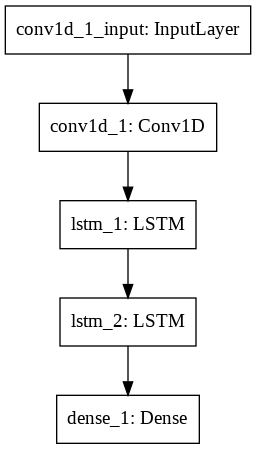
\includegraphics[width=0.3\textwidth]{figuras/fig4_2.png}
   \fonte{O autor.}
\end{figure}

O primeiro teste se concentrou no reconhecimento do tipo de superfície da vida. Foram reconhecidos três tipos diferentes, sendo pavimento rígido (asfalto), pavimento flexível (paralelepípedo ou hexagonal) e sem pavimentação (terra). A rede neural profunda para este reconhecimento obteve uma acurácia de 99\%, com um Erro Médio Quadrático (\textit{Mean Squared Error} - MSE) de 0.0000045885. O reconhecimento de pavimento asfáltico obteve o melhor resultado, com Erro Médio Absoluto (\textit{Mean Absolute Error} - MAE) de 0.000023. Em seguida, o reconhecimento de terra obteve MAE de 0.000054, e o reconhecimento de paralelepípedo/hexagonal obteve MAE de 0.000064. As Figuras \ref{fig:resultado_asfalto}, \ref{fig:resultado_paralelepipedo} e \ref{fig:resultado_terra} detalham os resultados.

O segundo teste foi voltado ao reconhecimento de lombadas. Sendo assim, envolveu lombadas tanto em pavimento asfáltico, quando em paralelepípedo, de diversas dimensões. A rede neural profunda para esse reconhecimento também obteve acurácia de 99\% e um MSE de 0.0005878024. O MAE foi de 0.000012, e os resultados são detalhados na Figura \ref{fig:resutlado_lombada}. Por fim, no terceiro teste foi realizado o reconhecimento de curvas à direita e à esquerda, sendo elas leves ou acentuadas. A rede obteve acurácia de 92\% com um MSE de 0.0020476580. Para curvas a esquerda, o MAE foi de 0.004028, e para a direita, de 0.010060. Os resultados são detalhados na Figura \ref{fig:resultado_curva_esquerda} e \ref{fig:resultado_curva_direita}.

De modo geral, é possível observar o bom desempenho a rede em filtrar sinais, extrair características e reconhecer os padrões, fazendo com que a LSTM seja interessante para este problema. Em relação à adaptabilidade, alguns fatores de dependência já foram agregados, como a velocidade e características sensoriais descritas na seção anterior. Sendo assim, faltam agregar os demais fatores ao modelo, e prosseguir com testes para outras percepções e outros contextos, com a produção de novos \textit{datasets}.

\begin{figure}[h!]
  \centering
  \caption{Reconhecimento de Pavimento Rígido (Asfalto).}
   \label{fig:resultado_asfalto}
   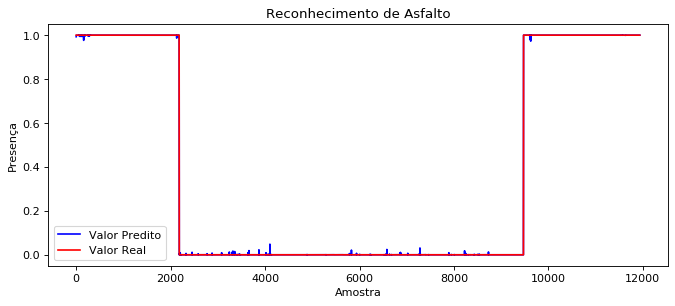
\includegraphics[width=1\textwidth]{figuras/fig4_2_1.png}
   \fonte{O autor.}
\end{figure}

\begin{figure}[h!]
  \centering
  \caption{Reconhecimento de Pavimento Flexível (Hexagonal ou Paralelepípedo).}
   \label{fig:resultado_paralelepipedo}
   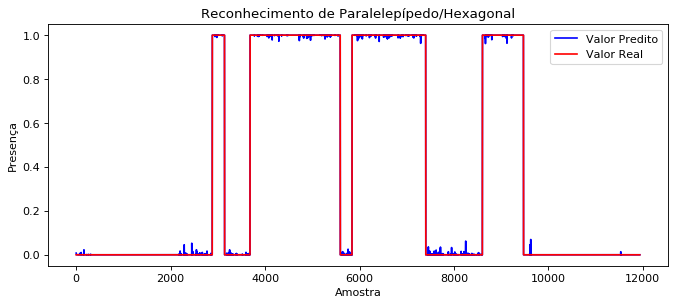
\includegraphics[width=1\textwidth]{figuras/fig4_2_2.png}
   \fonte{O autor.}
\end{figure}

\begin{figure}[h!]
  \centering
  \caption{Reconhecimento de Sem Pavimento (Terra).}
   \label{fig:resultado_terra}
   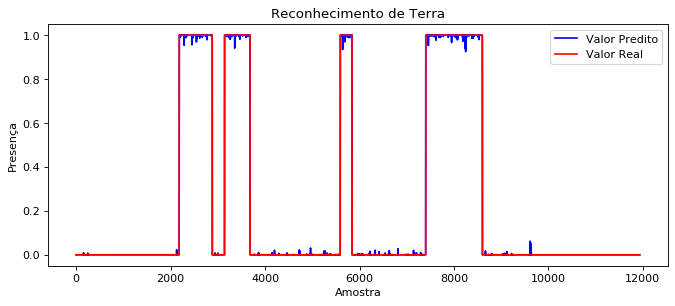
\includegraphics[width=1\textwidth]{figuras/fig4_2_3.png}
   \fonte{O autor.}
\end{figure}

\begin{figure}[h!]
  \centering
  \caption{Reconhecimento de Lombada.}
   \label{fig:resutlado_lombada}
   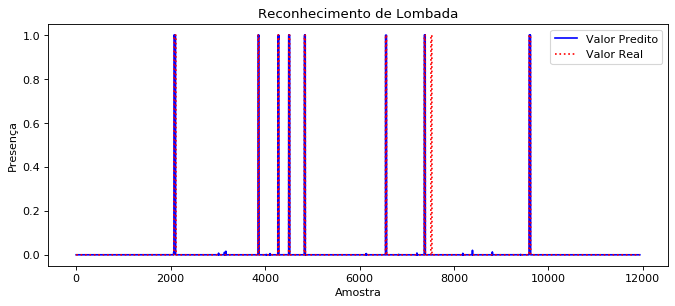
\includegraphics[width=1\textwidth]{figuras/fig4_2_4.png}
   \fonte{O autor.}
\end{figure}

\begin{figure}[h!]
  \centering
  \caption{Reconhecimento de Curva à Esquerda.}
   \label{fig:resultado_curva_esquerda}
   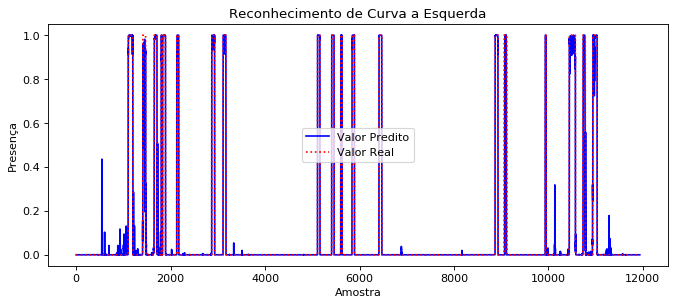
\includegraphics[width=1\textwidth]{figuras/fig4_2_5.png}
   \fonte{O autor.}
\end{figure}

\begin{figure}[h!]
  \centering
  \caption{Reconhecimento de Curva à Direita.}
   \label{fig:resultado_curva_direita}
   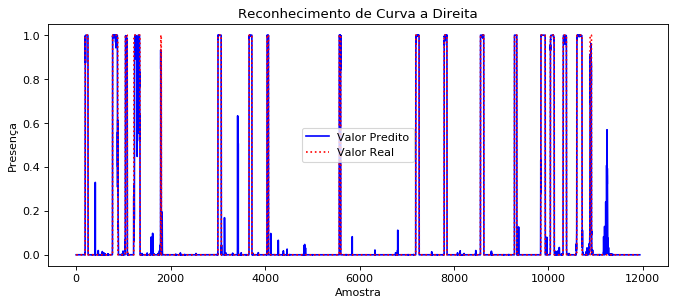
\includegraphics[width=1\textwidth]{figuras/fig4_2_6.png}
   \fonte{O autor.}
\end{figure}

\clearpage 
\section{Cronograma}

Abaixo é apresentado o cronograma a ser seguido com o intuito de cumprir as etapas da pesquisa e os requisitos que regulamentam o curso.

\begin{figure}[h!]
  \centering
  \caption{Cronograma de atividades.}
   \label{fig:proprioception_occurrence}
   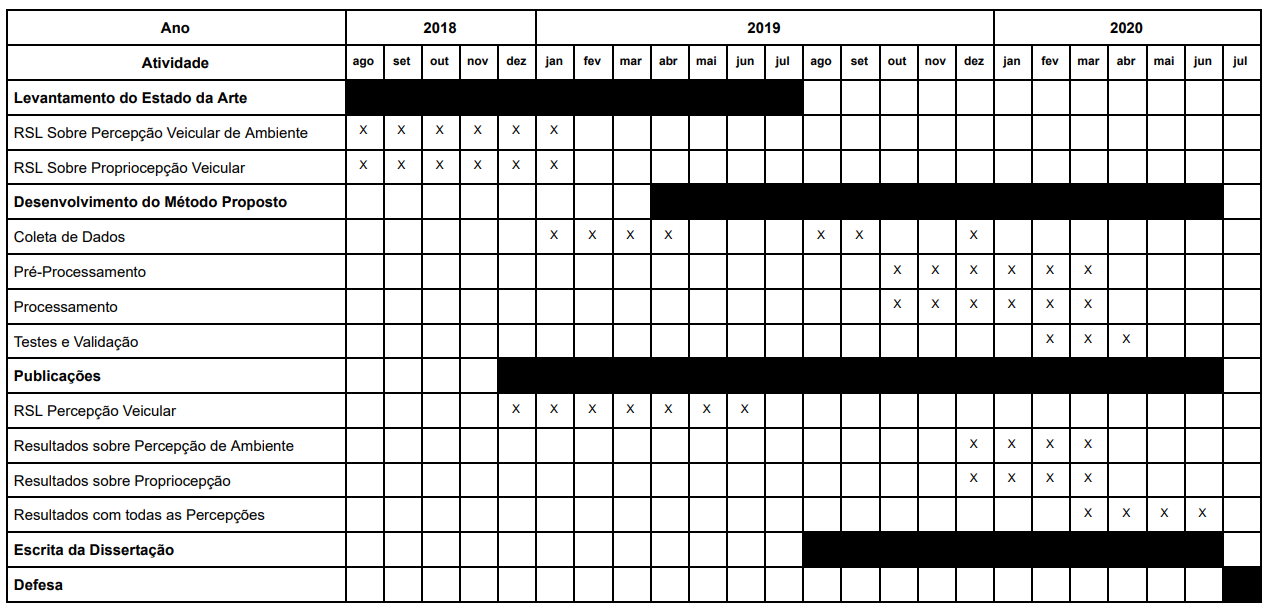
\includegraphics[width=1\textwidth]{figuras/fig4.png}
   \fonte{O autor.}
\end{figure}

